% Note that the a4paper option is mainly intended so that authors in
% countries using A4 can easily print to A4 and see how their papers will
% look in print - the typesetting of the document will not typically be
% affected with changes in paper size (but the bottom and side margins will).
% Use the testflow package mentioned above to verify correct handling of
% both paper sizes by the user's LaTeX system.
%
% Also note that the "draftcls" or "draftclsnofoot", not "draft", option
% should be used if it is desired that the figures are to be displayed in
% draft mode.
%
\documentclass[journal]{IEEEtran}
%
% If IEEEtran.cls has not been installed into the LaTeX system files,
% manually specify the path to it like:
% \documentclass[journal]{../sty/IEEEtran}


% Some very useful LaTeX packages include:
% (uncomment the ones you want to load)


% *** MISC UTILITY PACKAGES ***
%
\usepackage{glossaries}
\usepackage{booktabs} % to use \toprule


% *** CITATION PACKAGES ***
%
\usepackage[numbers]{natbib}
%\usepackage{cite}
% cite.sty was written by Donald Arseneau
% V1.6 and later of IEEEtran pre-defines the format of the cite.sty package
% \cite{} output to follow that of IEEE. Loading the cite package will
% result in citation numbers being automatically sorted and properly
% "compressed/ranged". e.g., [1], [9], [2], [7], [5], [6] without using
% cite.sty will become [1], [2], [5]--[7], [9] using cite.sty. cite.sty's
% \cite will automatically add leading space, if needed. Use cite.sty's
% noadjust option (cite.sty V3.8 and later) if you want to turn this off
% such as if a citation ever needs to be enclosed in parenthesis.
% cite.sty is already installed on most LaTeX systems. Be sure and use
% version 4.0 (2003-05-27) and later if using hyperref.sty. cite.sty does
% not currently provide for hyperlinked citations.
% The latest version can be obtained at:
% http://www.ctan.org/tex-archive/macros/latex/contrib/cite/
% The documentation is contained in the cite.sty file itself.






% *** GRAPHICS RELATED PACKAGES ***
%
\ifCLASSINFOpdf
  \usepackage[pdftex]{graphicx}
  % declare the path(s) where your graphic files are
  \graphicspath{{../2013-IPMI/Figures/}}
  % and their extensions so you won't have to specify these with
  % every instance of \includegraphics
  % \DeclareGraphicsExtensions{.pdf,.jpeg,.png}
\else
  % or other class option (dvipsone, dvipdf, if not using dvips). graphicx
  % will default to the driver specified in the system graphics.cfg if no
  % driver is specified.
  % \usepackage[dvips]{graphicx}
  % declare the path(s) where your graphic files are
  % \graphicspath{{../eps/}}
  % and their extensions so you won't have to specify these with
  % every instance of \includegraphics
  % \DeclareGraphicsExtensions{.eps}
\fi
% graphicx was written by David Carlisle and Sebastian Rahtz. It is
% required if you want graphics, photos, etc. graphicx.sty is already
% installed on most LaTeX systems. The latest version and documentation
% can be obtained at: 
% http://www.ctan.org/tex-archive/macros/latex/required/graphics/
% Another good source of documentation is "Using Imported Graphics in
% LaTeX2e" by Keith Reckdahl which can be found at:
% http://www.ctan.org/tex-archive/info/epslatex/
%
% latex, and pdflatex in dvi mode, support graphics in encapsulated
% postscript (.eps) format. pdflatex in pdf mode supports graphics
% in .pdf, .jpeg, .png and .mps (metapost) formats. Users should ensure
% that all non-photo figures use a vector format (.eps, .pdf, .mps) and
% not a bitmapped formats (.jpeg, .png). IEEE frowns on bitmapped formats
% which can result in "jaggedy"/blurry rendering of lines and letters as
% well as large increases in file sizes.
%
% You can find documentation about the pdfTeX application at:
% http://www.tug.org/applications/pdftex





% *** MATH PACKAGES ***
%
\usepackage[cmex10]{amsmath}
% A popular package from the American Mathematical Society that provides
% many useful and powerful commands for dealing with mathematics. If using
% it, be sure to load this package with the cmex10 option to ensure that
% only type 1 fonts will utilized at all point sizes. Without this option,
% it is possible that some math symbols, particularly those within
% footnotes, will be rendered in bitmap form which will result in a
% document that can not be IEEE Xplore compliant!
%
% Also, note that the amsmath package sets \interdisplaylinepenalty to 10000
% thus preventing page breaks from occurring within multiline equations. Use:
\interdisplaylinepenalty=2500
% after loading amsmath to restore such page breaks as IEEEtran.cls normally
% does. amsmath.sty is already installed on most LaTeX systems. The latest
% version and documentation can be obtained at:
% http://www.ctan.org/tex-archive/macros/latex/required/amslatex/math/

\usepackage{amssymb}
\DeclareMathOperator{\tr}{tr}
\DeclareMathOperator{\argmax}{argmax}
\DeclareMathOperator{\argmin}{argmin}
\DeclareMathOperator{\diag}{diag}
\DeclareMathOperator{\dist}{dist}
\DeclareMathOperator{\const}{Const.}
\providecommand{\e}[1]{\ensuremath{\times 10^{#1}}}



% *** SPECIALIZED LIST PACKAGES ***
%
\usepackage{algorithmic}
% algorithmic.sty was written by Peter Williams and Rogerio Brito.
% This package provides an algorithmic environment fo describing algorithms.
% You can use the algorithmic environment in-text or within a figure
% environment to provide for a floating algorithm. Do NOT use the algorithm
% floating environment provided by algorithm.sty (by the same authors) or
% algorithm2e.sty (by Christophe Fiorio) as IEEE does not use dedicated
% algorithm float types and packages that provide these will not provide
% correct IEEE style captions. The latest version and documentation of
% algorithmic.sty can be obtained at:
% http://www.ctan.org/tex-archive/macros/latex/contrib/algorithms/
% There is also a support site at:
% http://algorithms.berlios.de/index.html
% Also of interest may be the (relatively newer and more customizable)
% algorithmicx.sty package by Szasz Janos:
% http://www.ctan.org/tex-archive/macros/latex/contrib/algorithmicx/




% *** ALIGNMENT PACKAGES ***
%
%\usepackage{array}
% Frank Mittelbach's and David Carlisle's array.sty patches and improves
% the standard LaTeX2e array and tabular environments to provide better
% appearance and additional user controls. As the default LaTeX2e table
% generation code is lacking to the point of almost being broken with
% respect to the quality of the end results, all users are strongly
% advised to use an enhanced (at the very least that provided by array.sty)
% set of table tools. array.sty is already installed on most systems. The
% latest version and documentation can be obtained at:
% http://www.ctan.org/tex-archive/macros/latex/required/tools/


% IEEEtran contains the IEEEeqnarray family of commands that can be used to
% generate multiline equations as well as matrices, tables, etc., of high
% quality.




% *** SUBFIGURE PACKAGES ***
%\ifCLASSOPTIONcompsoc
%  \usepackage[caption=false,font=normalsize,labelfont=sf,textfont=sf]{subfig}
%\else
%  \usepackage[caption=false,font=footnotesize]{subfig}
%\fi
% subfig.sty, written by Steven Douglas Cochran, is the modern replacement
% for subfigure.sty, the latter of which is no longer maintained and is
% incompatible with some LaTeX packages including fixltx2e. However,
% subfig.sty requires and automatically loads Axel Sommerfeldt's caption.sty
% which will override IEEEtran.cls' handling of captions and this will result
% in non-IEEE style figure/table captions. To prevent this problem, be sure
% and invoke subfig.sty's "caption=false" package option (available since
% subfig.sty version 1.3, 2005/06/28) as this is will preserve IEEEtran.cls
% handling of captions.
% Note that the Computer Society format requires a larger sans serif font
% than the serif footnote size font used in traditional IEEE formatting
% and thus the need to invoke different subfig.sty package options depending
% on whether compsoc mode has been enabled.
%
% The latest version and documentation of subfig.sty can be obtained at:
% http://www.ctan.org/tex-archive/macros/latex/contrib/subfig/




% *** FLOAT PACKAGES ***
%
%\usepackage{fixltx2e}
% fixltx2e, the successor to the earlier fix2col.sty, was written by
% Frank Mittelbach and David Carlisle. This package corrects a few problems
% in the LaTeX2e kernel, the most notable of which is that in current
% LaTeX2e releases, the ordering of single and double column floats is not
% guaranteed to be preserved. Thus, an unpatched LaTeX2e can allow a
% single column figure to be placed prior to an earlier double column
% figure. The latest version and documentation can be found at:
% http://www.ctan.org/tex-archive/macros/latex/base/


%\usepackage{stfloats}
% stfloats.sty was written by Sigitas Tolusis. This package gives LaTeX2e
% the ability to do double column floats at the bottom of the page as well
% as the top. (e.g., "\begin{figure*}[!b]" is not normally possible in
% LaTeX2e). It also provides a command:
%\fnbelowfloat
% to enable the placement of footnotes below bottom floats (the standard
% LaTeX2e kernel puts them above bottom floats). This is an invasive package
% which rewrites many portions of the LaTeX2e float routines. It may not work
% with other packages that modify the LaTeX2e float routines. The latest
% version and documentation can be obtained at:
% http://www.ctan.org/tex-archive/macros/latex/contrib/sttools/
% Do not use the stfloats baselinefloat ability as IEEE does not allow
% \baselineskip to stretch. Authors submitting work to the IEEE should note
% that IEEE rarely uses double column equations and that authors should try
% to avoid such use. Do not be tempted to use the cuted.sty or midfloat.sty
% packages (also by Sigitas Tolusis) as IEEE does not format its papers in
% such ways.
% Do not attempt to use stfloats with fixltx2e as they are incompatible.
% Instead, use Morten Hogholm'a dblfloatfix which combines the features
% of both fixltx2e and stfloats:
%
% \usepackage{dblfloatfix}
% The latest version can be found at:
% http://www.ctan.org/tex-archive/macros/latex/contrib/dblfloatfix/




%\ifCLASSOPTIONcaptionsoff
%  \usepackage[nomarkers]{endfloat}
% \let\MYoriglatexcaption\caption
% \renewcommand{\caption}[2][\relax]{\MYoriglatexcaption[#2]{#2}}
%\fi
% endfloat.sty was written by James Darrell McCauley, Jeff Goldberg and 
% Axel Sommerfeldt. This package may be useful when used in conjunction with 
% IEEEtran.cls'  captionsoff option. Some IEEE journals/societies require that
% submissions have lists of figures/tables at the end of the paper and that
% figures/tables without any captions are placed on a page by themselves at
% the end of the document. If needed, the draftcls IEEEtran class option or
% \CLASSINPUTbaselinestretch interface can be used to increase the line
% spacing as well. Be sure and use the nomarkers option of endfloat to
% prevent endfloat from "marking" where the figures would have been placed
% in the text. The two hack lines of code above are a slight modification of
% that suggested by in the endfloat docs (section 8.4.1) to ensure that
% the full captions always appear in the list of figures/tables - even if
% the user used the short optional argument of \caption[]{}.
% IEEE papers do not typically make use of \caption[]'s optional argument,
% so this should not be an issue. A similar trick can be used to disable
% captions of packages such as subfig.sty that lack options to turn off
% the subcaptions:
% For subfig.sty:
% \let\MYorigsubfloat\subfloat
% \renewcommand{\subfloat}[2][\relax]{\MYorigsubfloat[]{#2}}
% However, the above trick will not work if both optional arguments of
% the \subfloat command are used. Furthermore, there needs to be a
% description of each subfigure *somewhere* and endfloat does not add
% subfigure captions to its list of figures. Thus, the best approach is to
% avoid the use of subfigure captions (many IEEE journals avoid them anyway)
% and instead reference/explain all the subfigures within the main caption.
% The latest version of endfloat.sty and its documentation can obtained at:
% http://www.ctan.org/tex-archive/macros/latex/contrib/endfloat/
%
% The IEEEtran \ifCLASSOPTIONcaptionsoff conditional can also be used
% later in the document, say, to conditionally put the References on a 
% page by themselves.




% *** PDF, URL AND HYPERLINK PACKAGES ***
%
\usepackage{url}
\usepackage{hyperref}
% url.sty was written by Donald Arseneau. It provides better support for
% handling and breaking URLs. url.sty is already installed on most LaTeX
% systems. The latest version and documentation can be obtained at:
% http://www.ctan.org/tex-archive/macros/latex/contrib/url/
% Basically, \url{my_url_here}.




% *** Do not adjust lengths that control margins, column widths, etc. ***
% *** Do not use packages that alter fonts (such as pslatex).         ***
% There should be no need to do such things with IEEEtran.cls V1.6 and later.
% (Unless specifically asked to do so by the journal or conference you plan
% to submit to, of course. )


% correct bad hyphenation here
\hyphenation{op-tical net-works semi-conduc-tor}

% -*- root: 00-main.tex -*-
% List of acronyms used in the text
\newacronym{mr}{MR}{magnetic resonance}
\newacronym{mri}{MRI}{magnetic resonance imaging}
\newacronym{dwi}{DWI}{diffusion weighted image}
\newacronym{dmri}{dMRI}{diffusion MRI}
\newacronym{dw}{DW}{diffusion weighted}
\newacronym{dti}{DTI}{diffusion tensor image}
\newacronym{t1}{T1w}{T1 weighted}
\newacronym{t2}{T2w}{T2 weighted}
\newacronym{csf}{CSF}{cerebrospinal fluid}
\newacronym{wm}{WM}{white matter}
\newacronym{gm}{GM}{grey matter}
\newacronym{epi}{EPI}{echo-planar imaging}
\newacronym{gre}{GRE}{gradient echo sequence}
\newacronym{fa}{FA}{fractional anisotropy}
\newacronym{md}{MD}{mean diffusivity}
\newacronym{adc}{ADC}{apparent diffusion coefficient}
\newacronym{acwe}{ACWE}{active contours without edges}
\newacronym{adf}{ADF}{active deformation field}
\newacronym{map}{MAP}{maximum a posteriori}
\newacronym{snr}{SNR}{signal-to-noise ratio}
\newacronym{pve}{PVE}{partial volume effect}
\newacronym{roi}{ROI}{region of interest}
\newacronym{mrf}{MRF}{Markov Random Field}
\newacronym{pde}{PDE}{partial differential equation}
\newacronym{swindex}{sWI}{surface warping index}
\newacronym{wi}{WI}{Warping index}
\newacronym{nof}{NoF}{number of fibers}
\newacronym{t2b}{T2B}{T2w-registration based}
\newacronym{fft}{FFT}{fast fourier transform}
\newacronym{hcp}{HCP}{Human Connectome Project}
\newacronym{pe}{PE}{phase-encoding}

\makeglossaries

%\acrodef{mr}[MR]{magnetic resonance}
%\acrodef{mri}[MRI]{magnetic resonance imaging}
%\acrodef{dwi}[DWI]{diffusion weighted imaging}
%\acrodef{dw}[DW]{diffusion weighted}
%\acrodef{dti}[DTI]{diffusion tensor imaging}
%\acrodef{t1}[T1]{T1-weighted}
%\acrodef{t2}[T2]{T2-weighted}
%\acrodef{csf}[CSF]{cerebrospinal fluid}
%\acrodef{wm}[WM]{white matter}
%\acrodef{gm}[GM]{grey matter}
%\acrodef{epi}[EPI]{echo-planar imaging}
%\acrodef{fa}[FA]{fractional anisotropy}
%\acrodef{md}[MD]{mean diffusivity}
%\acrodef{acwe}[ACWE]{active contours without edges}
%\acrodef{map}[MAP]{maximum a posteriori}
%\acrodef{snr}[SNR]{signal-to-noise ratio}
%\acrodef{pve}[PVE]{partial volume effect}
%\acrodef{roi}[ROI]{region of interest}



\begin{document}
%
% paper title
% can use linebreaks \\ within to get better formatting as desired
% Do not put math or special symbols in the title.
\title{A variational framework for distortion correction,
       segmentation and cortical parcellation of diffusion MRI}
%
%
% author names and IEEE memberships
% note positions of commas and nonbreaking spaces ( ~ ) LaTeX will not break
% a structure at a ~ so this keeps an author's name from being broken across
% two lines.
% use \thanks{} to gain access to the first footnote area
% a separate \thanks must be used for each paragraph as LaTeX2e's \thanks
% was not built to handle multiple paragraphs
%
\author{Oscar~Esteban$^{*}$,~\IEEEmembership{Member,~IEEE,}
        Alessandro~Daducci,~\IEEEmembership{Member,~IEEE,}
        Meritxell~Bach-Cuadra,~\IEEEmembership{Member,~IEEE,}
        Jean-Philippe~Thiran,~\IEEEmembership{Member,~IEEE,}
        Andr\'es~Santos,~\IEEEmembership{Member,~IEEE,}
        and~Dominique~Zosso,~\IEEEmembership{Life~Fellow,~IEEE}% <-this % stops a space
\thanks{Manuscript received XXX XX, 2013; revised XXX XX, 2013.
This study is supported by: the Spain's Ministry of Science and Innovation 
(projects TEC2010-21619- C04-03, TEC2011-28972-C02-02, CDTI-CENIT
AMIT and INNPACTO PRECISION), Comunidad de Madrid (ARTEMIS) and
European Regional Development Funds; the Center for Biomedical Imaging
(CIBM) of the Geneva and Lausanne Universities and the EPFL, as well as the
Leenaards and Louis Jeantet foundations.\emph{~Asterisk indicates corresponding
author}.}%
\thanks{$^{*}$O. Esteban is with the Biomedical Image Technologies (BIT), ETSI Telecomunicaci\'on,
Universidad Polit\'ecnica de Madrid and CIBER-BBN, Madrid, Spain,
and the Signal Processing Laboratory (LTS5), \'Ecole Polytechnique
F\'ed\'erale de Lausanne (EPFL), Lausanne, Switzerland (e-mail: phd@oscaresteban.es).}% <-this % stops a space
\thanks{A. Daducci is with the Signal Processing Laboratory (LTS5), \'Ecole Polytechnique
F\'ed\'erale de Lausanne (EPFL), Lausanne, Switzerland.}%
\thanks{M. Bach-Cuadra and JP. Thiran are with the Signal Processing Laboratory (LTS5), \'Ecole Polytechnique
F\'ed\'erale de Lausanne (EPFL), Lausanne, Switzerland, and Dept. of Radiology, University
Hospital Center (CHUV) and University of Lausanne (UNIL), Lausanne, Switzerland.}%
\thanks{A. Santos is with the Biomedical Image Technologies (BIT), ETSI Telecomunicaci\'on,
Universidad Polit\'ecnica de Madrid and CIBER-BBN, Madrid, Spain.}% <-this % stops a space
\thanks{D. Zosso is with the Department of Mathematics, University of California, 
Los Angeles (UCLA), Los Angeles, CA, US and is supported by the Swiss National 
Science Foundation (SNF) under grant PBELP2-137727.}% <-this % stops a space
}

% note the % following the last \IEEEmembership and also \thanks - 
% these prevent an unwanted space from occurring between the last author name
% and the end of the author line. i.e., if you had this:
% 
% \author{....lastname \thanks{...} \thanks{...} }
%                     ^------------^------------^----Do not want these spaces!
%
% a space would be appended to the last name and could cause every name on that
% line to be shifted left slightly. This is one of those "LaTeX things". For
% instance, "\textbf{A} \textbf{B}" will typeset as "A B" not "AB". To get
% "AB" then you have to do: "\textbf{A}\textbf{B}"
% \thanks is no different in this regard, so shield the last } of each \thanks
% that ends a line with a % and do not let a space in before the next \thanks.
% Spaces after \IEEEmembership other than the last one are OK (and needed) as
% you are supposed to have spaces between the names. For what it is worth,
% this is a minor point as most people would not even notice if the said evil
% space somehow managed to creep in.



% The paper headers
\markboth{IEEE TRANSACTIONS ON MEDICAL IMAGING,~Vol.~??, No.~?, MAY~2013}%
{Esteban \MakeLowercase{\textit{et al.}}: FIXME: Running title}
% The only time the second header will appear is for the odd numbered pages
% after the title page when using the twoside option.
% 
% *** Note that you probably will NOT want to include the author's ***
% *** name in the headers of peer review papers.                   ***
% You can use \ifCLASSOPTIONpeerreview for conditional compilation here if
% you desire.




% If you want to put a publisher's ID mark on the page you can do it like
% this:
%\IEEEpubid{0000--0000/00\$00.00~\copyright~2012 IEEE}
% Remember, if you use this you must call \IEEEpubidadjcol in the second
% column for its text to clear the IEEEpubid mark.



% use for special paper notices
%\IEEEspecialpapernotice{(Invited Paper)}




% make the title area
\maketitle

% As a general rule, do not put math, special symbols or citations
% in the abstract or keywords.
\begin{abstract}
% -*- root: 00-main.tex -*-
Current methods for processing \gls*{dmri} to map the connectivity of the human brain
  require precise delineations of anatomical structures.
\revcomment[C1 (R.1)]{%
The requirement has been approached either segmenting the data in native \gls*{dmri} space
  or projecting the structural information from \gls*{t1} images.
The characteristic features of diffusion data in terms of \acrlong*{snr}, resolution, etc.
  and the geometrical distortions caused by the inhomogeneity of magnetic susceptibility
  across tissues render the problem challenging.}
\revcomment[C10 (R.2)]{%
To solve the problem in a unified approach, we propose \regseg{}, a surface-to-volume nonlinear
  registration method that segments homogeneous regions within multivariate images by mapping
  a set of nested reference-surfaces.}
\revcomment[C11 (R.2)]{%
The surfaces can be extracted from the \gls*{t1} image of the subject, and the target image
  is the bivariate volume comprehending the \gls*{fa} and the \gls*{adc} maps derived from the
  \gls*{dmri} dataset.}
We first verify the subpixel accuracy of \regseg{} on digital phantoms, to then propose an
  evaluation framework that uses \gls*{dmri} datasets from the \gls*{hcp}.
In this framework, the undistorted \gls*{dmri} undergo a known distortion derived from real
  fieldmaps.
We analyze the misregistration error of the surfaces estimated by \regseg{} on 16 datasets.
The distribution of errors shows a 95\% CI of 0.56--0.66 mm, below the \gls*{dmri} resolution
  (1.25 mm, isotropic).
Finally, we cross-compare the proposed tool against a nonlinear \lowb{}-to-T2w registration
  method, thereby obtaining a significantly lower misregistration error with \regseg{}.
\end{abstract}

% Note that keywords are not normally used for peerreview papers.
\begin{IEEEkeywords}
diffusion MRI,~susceptibility~distortion,~segmentation,~registration,~parcellation,~shape-prior.
\end{IEEEkeywords}






% For peer review papers, you can put extra information on the cover
% page as needed:
% \ifCLASSOPTIONpeerreview
% \begin{center} \bfseries EDICS Category: 3-BBND \end{center}
% \fi
%
% For peerreview papers, this IEEEtran command inserts a page break and
% creates the second title. It will be ignored for other modes.
\IEEEpeerreviewmaketitle


% -*- root: 00-main.tex -*-
\section{Introduction}\label{sec:regseg-intro}
\Acrlong*{dmri} enables the mapping of microstructure \citep{basser_microstructural_1996}
  and connectivity \citep{craddock_imaging_2013} of the human brain \emph{in-vivo}.
It is generally acquired using \gls*{epi} schemes, since they are very fast at
  scanning a large sequence of images called \glspl*{dwi}.
Each \gls*{dwi} is sensitized with a gradient to probe proton diffusion in a certain
  orientation.
Subsequent processing involves describing the local microstructure with one of the available
  models, which range from the early \gls*{dti} proposed by \cite{basser_microstructural_1996}
  to current models such as \gls*{amico}.
The microstructural map is then used to draw the preferential orientations of diffusion
  across the brain using tractography \citep{mori_threedimensional_1999}.
Finally, a graph representing the corresponding structural network is built using
  the regions of a cortical parcellation as nodes and the fiber paths found by
  tractography as edges \citep{hagmann_mapping_2008}.
The methodologies to solve reconstruction, tractography and network building
  require the delineation of the anatomy in the \gls*{dmri} space.
Moreover, current trends on reconstruction \citep{jeurissen_multitissue_2014} and
  tractography \citep{smith_anatomicallyconstrained_2012} are increasingly using
  structural information to improve the microstructural mapping and fiber-tracking.

Possibly, the earliest structural information incorporated to aid \gls*{dmri} processing
  is the \gls*{wm} mask used as a termination criteria for tractography.
The standardized procedure to obtain this mask was thresholding the \gls*{fa} map.
However, the mask and subsequent analyses are highly dependent on the 
  threshold that is chosen \citep{taoka_fractional_2009}.
To overcome the unreliability of \gls*{fa} thresholding, and to broaden
  \gls*{wm} segmentation to brain tissue segmentation, a large number of
  methods have been proposed using \glspl*{dwi}, the \lowb{}, and \gls*{dti}-derived
  scalar maps such as \gls*{fa}, \gls*{adc} and others \citep{zhukov_level_2003,
  rousson_level_2004,jonasson_segmentation_2005,hadjiprocopis_unbiased_2005,liu_brain_2007,
  lu_segmentation_2008,han_experimental_2009}.
However, the precise segmentation of \gls*{dmri} is difficult for several reasons.
First, \gls{dmri} images have a resolution that is much lower
  than that of the imaged microstructural features.
Therefore, voxels located in structural discontinuities are affected by partial
  voluming of the signal sources.
Second, the extremely low \gls*{snr} and the high dimensionality of the \glspl*{dwi} prevent
  their direct use in segmentation.
Third, the low contrast between \gls*{gm} and \gls*{wm} in the \lowb{} volume also makes
  it unsuitable for brain tissue segmentation.

An alternative route to segmentation in \gls*{dmri} space is the mapping of the
  structural information extracted from anatomical MR images, such as \gls*{t1}, using
  image registration techniques.
Generally, intra-subject registration of MR images of the brain involves only a linear
  mapping to compensate for head motion between scans.
However, \gls*{epi} introduces a geometrical distortion \citep{jezzard_correction_1995}
  that impedes the linear mapping from the structural space.
Numerous methods have been proposed to overcome this problem by incorporating information
  from extra MR acquisitions such as fieldmaps \citep{jezzard_correction_1995},
  \glspl*{dwi} with a different \gls*{pe} scheme \citep{cordes_geometric_2000,chiou_simple_2000},
  or \gls*{t2} images \citep{kybic_unwarping_2000,studholme_accurate_2000}.
These methods estimate the deformation field associated to \emph{\gls*{epi} distortions} and
  resample the \glspl*{dwi} onto a corrected \gls*{dmri} space.
The retrospective \gls*{epi} correction is an active field of research yielding frequent refinements
  and combinations of the original methods, such as
  \citep{holland_efficient_2010,andersson_comprehensive_2012,
  irfanoglu_drbuddi_2015}.
A standardized method to solve the remaining linear mapping between the corrected-\gls*{dmri}
  and the structural spaces is \emph{bbregister} \citep{greve_accurate_2009}.

Here, we present a segmentation and surface-to-volume registration method
  called \regseg{}, and show its usefulness in mapping anatomical information from structural
  space into native \gls*{dmri} space to aid subsequent processing steps
  (reconstruction, tractography and network building using a cortical parcellation).
The underlying hypothesis is that the registration and segmentation problems
  in \gls*{dmri} can be solved simultaneously.
To implement \regseg{} we first establish an active-contours without edges
  \citep{chan_active_2001} segmentation framework.
A specific set of reference surfaces extracted from the same subject initialize
  the 3D active contours, which evolve searching for homogeneous regions in the multivariate
  target-image.
We apply \regseg{} to segment \gls*{dmri} data by mapping
  a set of nested surfaces extracted from a structural image (e.g. \gls*{t1}) to
  a bivariate target-volume comprehending the \gls*{fa} and \gls*{adc} maps.
The evolution of the surfaces is supported by a B-spline basis, optimized
  iteratively using a descent approach driven by shape-gradients
  \citep{besson_dream2s_2003,herbulot_segmentation_2006}.
Therefore, \regseg{} establishes a registration framework that actually
  deals with the nonlinear warping induced by \gls*{epi} distortions.
\Regseg{} integrates the benefits of segmentation and registration methods together and
  exploits the multivariate nature of \gls*{dmri} data to contribute in the proposed
  application on three key aspects:
  1) the surfaces are typically extracted from the \gls*{t1} image of the same subject,
    therefore \regseg{} does not require additional MR acquisitions to the minimal
    \gls*{dmri} protocol in order to estimate the deformation field;
  2) \revcomment[R\#1-C2]{%
    alternatively to the typical design of the processing flow, the information from the
    reference \gls*{t1} can precisely be mapped onto the distorted \gls*{dmri} space,
    avoiding the interpolation of the \glspl*{dwi} required by unwarping the diffusion data; and} 
%    depending on the application, the resampling of the \glspl*{dwi}
%    introduced by the correction method can be avoided, either by performing the posterior
%    processing on the native \gls*{dmri} space or applying the unwarping on the tractography
%    itself; and
  3) \regseg{} increases the geometrical accuracy of the overall process.
In this paper, we first verify the functionality of the method and the \regseg{}
  implementation using a set of digital phantoms, demonstrating the
  \revcomment[R\#3-C10]{subvoxel} accuracy in registration.
Then, we evaluate \regseg{} on real \gls*{dmri} datasets, using a derivation of our
  instrumentation framework \citep{esteban_simulationbased_2014} which simulates
  known and realistic \gls*{epi} distortions.
We also compare \regseg{} and a nonlinear registration method to map the \lowb{} to
  the corresponding \gls*{t2} image of the same subject.
This approach is the first step of the \gls*{t2b} correction
  methods \citep{kybic_unwarping_2000}.
We reproduce the settings and implementation of a widely used diffusion
  processing software \citep[\emph{ExploreDTI},][]{leemans_exploredti_2009}.
With this comparison, we demonstrate how \regseg{} achieves higher accuracy with the
  simultaneous registration and segmentation process.

\section{Methods}
\label{sec:methods}
%
\subsection{Related work}
\label{sec:methods_background}

\Gls{acwe} and level-set based formulations have been widely applied in image
processing, as reviewed in \citep{suri_shape_2002}. We suggest clustering the 
current methodologies of template-based segmentation methods into three groups. 
The first group typically adds a shape prior term to the energy functional of 
an evolving active contour \citep{bresson_variational_2006,
chan_level_2005,chen_using_2002,cremers_kernel_2006,gastaud_combining_2004}.
These methods generally have an explicit description of the expected relative boundary 
locations of the object to be delineated, and some even model the statistical deviations
from this average shape. By including a coordinates mapping, it is possible to perform
active contours based registration between timesteps in a time-series or between different
images \citep{bertalmio_morphing_2000,wyatt_map_2003,paragios_level_2003,vemuri_joint_2003,
yezzi_variational_2003}.
A summary of these second set of techniques is performed in \citep{droske_mumfordshah_2009},
proposing two different approaches to applying the Mumford-Shah \citep{mumford_optimal_1989}
functional in joint registration and segmentation. Finally, a derivation of the 
latter groups is composed by atlas-based segmentation methods 
\citep{gorthi_segmentation_2009,gorthi_active_2011,pohl_unifying_2005,
pohl_bayesian_2006,wang_joint_2006}, where the prior 
imposes consistent voxel-based classification of contiguous regions.
A comprehensive summary of the \gls{acwe}-derived methodologies with special attention
to joint registration-segmentation methods is found in \citep{gorthi_active_2011}.

Our joint registration and segmentation method is mainly inspired in the active
deformation fields presented by \citep{gorthi_active_2011}, that is a generalization
of the methodologies under second and third groups before. As it is described in
their work, the first joint ``morphing''-segmentation approach (it was not a proper
registration method) was proposed in \citep{bertalmio_morphing_2000}. The first
registration framework is presented by \citep{yezzi_variational_2001} where the
energy functional is defined simultaneously in the moving and target images with
an affine transformation supporting the coordinates mapping (``2 PDEs approach'').
\citep{vemuri_joint_2003} proposed the first atlas-based registration based on the 
level set framework and using only one PDE. \citep{unal_coupled_2005} extended the 
idea of \citep{bertalmio_morphing_2000,yezzi_variational_2001} for non-linear 
registration with a dense deformation field as mapping function. \citep{droske_mumfordshah_2009}
combining ideas from both branches and proposed the propagation of the 
deformation field from the contours to the whole image definition. Finally,
\citep{gorthi_active_2011} present a comprehensive generalization of the methodologies.

All the surveyed frameworks are deduced from the general level set evolution equation
introduced by \citep{osher_fronts_1988}:
\begin{equation}
\frac{\partial \Phi_D(\mathbf{x},t)}{\partial t} = \nu ( \Phi_D(\mathbf{x},t)) \, \left| \nabla \Phi_D(\mathbf{x},t) \right|
\end{equation}
where $\nu$ is the velocity of the flow or speed function that contains the local
segmentation and contour regularization constraints, and $\Phi_D: \Omega \to \mathbb{R}$
is the signed distance function often used to represent implicitly the active contour
by its zero level. An early extension to image registration was proposed by 
\citep{vemuri_joint_2003} but replacing $\Phi_D$ by the intensity function of the
image to register, $\Phi_I: \Omega \to \mathbb{R}$ (the moving image). 
\citep{bertalmio_morphing_2000,vemuri_joint_2003} then define the speed function as
$\nu(\Phi_I(\mathbf{x},t)) = \Phi_I(\mathbf{x},t) - \Phi_T(\mathbf{x},t)$, where $\Phi_T(\mathbf{x})$ is the intensity
function of the target image. Finally, \citep{gorthi_active_2011} propose a different
multiphase label function as level set function ($\Phi_L$) that improves registration
results.

Naming $\Phi_G$ a generic objective function, a dense deformation field of vectors 
$u: \mathbb{R}^n \to \mathbb{R}^n$ (tipically $n = \{ 2, 3 \}$) is introduced. 
Then, the conservation of the morphological description is assumed, such as
$\Phi_G(\mathbf{x},t) = \Phi_G( \mathbf{x} + du, t + dt ) \implies d\Phi_G(\mathbf{x},t) = 0$, where $d\Phi_G$ is
the total derivative of $\Phi_G$. Using the chain rule, it can be rewritten as the 
evolution equation of a vector flow:
\begin{equation}
\frac{\partial u(\mathbf{x},t)}{\partial t}= - \frac{\Phi_G}{\left| \nabla \Phi_G \right|} N_{\Phi_G},
\end{equation}
where $N_{\Phi_G}$ is the normal of the level set. Finally, they introduce the general
level set evolution equation into the vector flow to perform the registration task:
\begin{equation}
\frac{\partial u(\mathbf{x},t)}{\partial t} = - \nu( \Phi_G(\mathbf{x},t) ) N_{\Phi_G}.
\end{equation}
Therefore, the position of the level set function $\Phi_G$ at time $t$ is given by the
deformation field $u(\mathbf{x},t)$ and the initial level set function $\Phi_G(\mathbf{x},0)$, yielding:
\begin{equation}
\frac{\partial u(\mathbf{x},t)}{\partial t} = - \nu( \Phi_G(\mathbf{x} + u(\mathbf{x},t), 0) ) N_{\Phi_G}.
\end{equation}

Here, we propose an active deformation field framework with some differences in
the formulation of the problem. The main diverging points with respect to
\citep{gorthi_active_2011} are: 1) there is no need for an explicit level set function
$\Phi_G$, as we replace the level set gradient computation $N_{\Phi_G}$ with shape
gradients \citep{jehan-besson_dream2s:_2003,herbulot_segmentation_2006}; 2) 
\todo[inline]{regularization is also based on linear diffusion smoothing REF-thirion,
but they use a Gaussian filtering)}; 3) optimization is applied in the spectral
domain, observing anisotropic and inhomogeneous mappings along each direction.


\subsection{Bridging segmentation frameworks}
\label{sec:methods_map}
%
A widely used approach to image segmentation is derived from the
Bayes' rule \eqref{eq:bayes_rule}. This framework seeks for a 
partitioning of a certain observation of features $F: \mathbb{R}^n \to %
\mathbb{R}^C$ (an $n$-dimensional \emph{image} comprising $C$ different 
channels) in piecewise smooth regions $\Omega = \lbrace \Omega_k , 
k\in\left[ 1 \ldots K \right] \rbrace$,  that maximize the \emph{a posteriori}
probability $p(\Omega \mid F)$:
\begin{equation}
p(\Omega \mid F) = \frac{p(F \mid \Omega)\, p(\Omega)}{p(F)},
\label{eq:bayes_rule}
\end{equation}
where $p(F \mid \Omega)$ is the \emph{likelihood} of the realization 
of $F$ given a certain region set $\Omega$. The second term, $p(\Omega)$,
is the a-priori probability of the partitioning. Finally, $p(F)$ is the 
probability of a certain image realization, and thus, it will remain 
constant when computing the \gls{map}. Consequently, the Bayes' rule
can be simplified for the optimization as follows:
\begin{equation}
p(\Omega \mid F) \propto p(F \mid \Omega)\, p(\Omega).
\label{eq:bayes_rule_simplified}
\end{equation}

In the simplest Bayesian segmentation framework, the unknown is the
parameter set $\Theta_k$ of region-wise descriptors that minimize 
\eqref{eq:bayes_rule}. Conversely, we can assume these descriptors as
fixed (fulfilling the concept of conservation of morphological description
mentioned before) and introduce a realization of a dense deformation field $U: %
\mathbb{R}^n \to \mathbb{R}^n$ that maps the initial partition $\Omega_0$
to the estimated one:
\begin{equation}
\Omega' = \Omega_0 + \hat{U}.
\label{eq:omega_tf}
\end{equation}

Thus, \eqref{eq:bayes_rule_simplified} is rewritten as 
$p(U \mid F) \propto p(F \mid U)\, p(U)$ that yields the
following \gls{map} solution:

\begin{equation}
\hat{U} = \underset{U}{\argmax} \left\{ p(U \mid F) \right\} = 
\underset{U}{\argmax} \left\{ p(F \mid U)\, p(U) \right\}.
\label{eq:map_u}
\end{equation}


An extended assumption is that the feature vector realization $F$ is
\emph{i.i.d.}, and thus, it is possible to write the a-posteriori
probability $p(F \mid U)$ as a continuous product with $d\mathbf{x}$ the
infinitesimal voxel size:
\begin{equation}
p(F \mid U) \, p(U) = \underset{k}{\prod} \underset{\mathbf{x}\in \Omega'_k}{\prod}
p_k\left( F(\mathbf{x} + U(\mathbf{x})) \mid U(\mathbf{x}) \right)^{d\mathbf{x}}.
\label{eq:bayes_aposteriori}
\end{equation}
\todo[inline]{I'm not convinced about turning $p(\Omega)$ into $p(U)$.}

A second widely-accepted assumption is the multivariate normal 
distribution of the different tissues in \gls{mri} data. Therefore,
the posterior probability of an infinitesimal voxel can be written as:
\begin{equation}
p_k( F(\mathbf{x}) \mid U(\mathbf{x}) ) = \frac{1}{ \sqrt{(2\pi)^{C}\,\left|\boldsymbol{\Sigma}_{k}\right|}}\,{e^{\left(-\frac{1}{2}  \Delta^2_k (\mathbf{f}') \right)}}.
\label{eq:bayes_mpdf}
\end{equation}
where we can identify the factor in the exponential as the squared \emph{Mahalanobis 
distance} of the feature observed in the displaced position, $\mathbf{f}' = 
F(\mathbf{x} + U(\mathbf{x}))$ with region descriptors
$\Theta_k = \lbrace \boldsymbol{\mu}_k, \boldsymbol{\Sigma}_k \rbrace$:
\begin{equation}
\Delta^2_k (\mathbf{f} \mid \Theta_k ) = (\mathbf{f} - \boldsymbol{\mu}_k)^T \, \boldsymbol{\Sigma}^{-1}_k \, (\mathbf{f} - \boldsymbol{\mu}_k).
\label{eq:bayes_mahalanobis}
\end{equation}

Finally, we can turn the \gls{map} problem into a variational one
applying the following log-transform:
\begin{multline}
E(F \mid U)= -\log \left[ p(F \mid U) \, p(U) \right] = \\
= -\log \left[ \underset{k}{\prod} \underset{\mathbf{x}\in \Omega'_k}{\prod}
p_k( F(\mathbf{x}) \mid U(\mathbf{x}) )^{d\mathbf{x}} \right] = \\
= \sum\limits_k \int_{\Omega'_k} -\log \left[ p_k(F(\mathbf{x}) \mid U(\mathbf{x} ) ) \right] \, d\mathbf{x},
\label{eq:energy_1}
\end{multline}
and introducing the posterior probability term \eqref{eq:bayes_mpdf}, 
we can express the functional in terms of the deformation field $U$ and
the region descriptors $\Theta_k$:
\begin{multline}
E(U) = \\
= \sum\limits_k \int_{\Omega'_k} -\log \left[ \frac{1}{ \sqrt{(2\pi)^{C}\,\left|\boldsymbol{\Sigma}_{k}\right|}}\,{e^{\left(-\frac{1}{2}  \Delta^2_k (\mathbf{f}) \right)}} \right] \, d\mathbf{x} = \\
= \sum\limits_k \int_{\Omega'_k} \left[ \frac{1}{2} \log{ \left( (2\pi)^{C}\,\left|\boldsymbol{\Sigma}_{k}\right| \right)} + \frac{1}{2}  \Delta^2_k (\mathbf{f}) \right] \,d\mathbf{x}.
\end{multline}
Finally, after removing scaling factors and independent constants,
we obtain:
\begin{align}
E(U) = \sum\limits_k \left[ \left|\Omega'_k\right|\,\log \left|\mathbf{\Sigma}_k \right| + \int_{\Omega'_k} \Delta^2_k (\mathbf{f}) \,d\mathbf{x} \right],
\label{eq:map_energy}
\end{align}
where we have a constant term scaled by the total volume of the partition $\Omega_k$ and 
the determinant of the  covariance matrix of the partition $\left|\boldsymbol{\Sigma}_{k}\right|$,
plus an energy term based on the squared \emph{Mahalanobis distance}.
As long as this shape-based registration framework is designed to allow small changes
between boundaries (and therefore, their volumes), and the shape descriptors should not
change significantly due to the conservation principle, the first term can be optionally
dismissed with respect the second one, what yields:
\begin{align}
E(U) = \sum\limits_k \int_{\Omega'_k} \Delta^2_k (\mathbf{f}) \,d\mathbf{x}.
\label{eq:final_map_energy}
\end{align}

This latter expression resembles the Mumford-Shah functional 
\citep{mumford_optimal_1989} which is at the background of all \gls{acwe}-based
methods. In this case, \eqref{eq:final_map_energy} includes covariance as
region descriptor, what modifies the original functional in a way that it 
can deal with more general distributions. This is necessary to avoid the 
assumption that regions $\Omega_k$ have a fixed covariance matrix on their 
complete domain. One immediate advantage of this functional from the original 
one is the possibility to distinguish regions with the same mean vector but 
different covariance matrix \citep{brox_local_2009}. In this work, the 
Mumford-Shah functional is derived for this extension as follows:
\begin{multline}
E(\Theta_k,\Omega_k) = \sum\limits_k \int_{\Omega_k} \left[ \log \left|\mathbf{\Sigma}_k\right| + \Delta^2_k (\mathbf{f}) \right] \,d\mathbf{x} \\
+ \lambda \int_{\Omega_k - K}  ( \left| \nabla \mathbf{\mu} \right| ^2 + \left| \nabla \mathbf{\Sigma}_k \right| ^2 ) \, d\mathbf{x} 
+ \nu |K|,
\end{multline}
that is easily identifiable with \eqref{eq:map_energy} when we apply 
the so-called \emph{cartoon limit}, 
for $\lambda \to \infty$:
\begin{equation}
E(\Theta_k,K) = \sum\limits_k \int_{\Omega_k} \left[ \log \left|\mathbf{\Sigma}_k\right| + \Delta^2_k (\mathbf{f}) \right] \,d\mathbf{x}
+ \nu |K|.
\end{equation}

As long as we do not penalize the edge set $K$ length, $\nu = 0$ and
the result is dual to \eqref{eq:map_energy}:
\begin{equation}
E(\Theta_k,K) = \sum\limits_k \int_{\Omega_k} \left[ \log \left|\mathbf{\Sigma}_k\right| + \Delta^2_k (\mathbf{f}) \right] \,d\mathbf{x}.
\end{equation}


\subsection{Introducing priors}
\label{sec:priors}
%
By introducing $U$ in \eqref{eq:bayes_rule_simplified}, we transformed 
the segmentation problem into a registration one provided with $\Omega_0$ 
(the initial partition) is derived from the shape-priors given in reference 
space. Therefore, the priors can be expressed in terms of the deformation
field:
\begin{equation}
P(U) = \underset{\mathbf{x}}{\prod}\,p(U(\mathbf{x}))\,^{d\mathbf{x}}.
\label{eq:prior_u}
\end{equation}
We define $P(U(\mathbf{x})) = p(\mathbf{u}) = \underset{d}\prod \, p_d(\mathbf{u})$ 
with $d$ the order of the derivative. We also assume that an initial
affine registration let us consider that the deformation field ($d=0$)
and its derivatives up to some order ($d>0$) are all zero mean, and
have some variance $\Sigma_d$. We restrict ourselves to $d=\lbrace 0,1 \rbrace$
(the field and its gradient):
\begin{subequations}
\begin{equation}
p_0(\mathbf{u}) = \mathcal{N}( \mathbf{u} \mid 0, \alpha^{-1}),
\end{equation}
\begin{equation}
p_1(\mathbf{u}) = \mathcal{N}( \nabla \mathbf{u} \mid 0, {\Sigma_\beta}^{-1}), 
\end{equation}
\end{subequations}
And therefore:
\begin{equation}
P(U) = \underset{\mathbf{x}}\prod \left[ p_0(\mathbf{u}) \, p_1(\mathbf{u}) \right]^{d\mathbf{x}}.
\end{equation}




\subsection{Numerical Implementation}
%
Let us denote $\{c_i\}_{i=1 \ldots N_c}$ the nodes of one or several shape-prior
surface(s). In our application, precise tissue interfaces of interest 
extracted from a high-resolution, anatomically correct reference volume. 
On the other hand, we have a number of \gls{dwi}-derived features at each
voxel of the volume. Let us denote by $\mathbf{x}$ the voxel and $f(\mathbf{x}) = 
[ f_1, f_2, \ldots, f_N]^T(\mathbf{x})$ its associated feature vector.

\subsubsection{Deformation field}
\label{sec:deformation_field}
The transformation from reference into \gls{dwi} coordinate space is 
achieved through a dense deformation field $u(\mathbf{x})$, such that:
\begin{equation}
c_i' = T\{c_i\} = c_i + u(c_i),
\end{equation}
what is equivalent to \eqref{eq:omega_tf}. Since the nodes of the anatomical 
surfaces might lay off-grid, it is required to derive $u(\mathbf{x})$ from a discrete 
set of parameters $\{u_k\}_{k=1 \ldots K}$. Densification is achieved through 
a set of associated basis functions $\psi_k$ (e.g. rbf, interpolation splines):
%
\begin{equation}
u(\mathbf{x}) = \sum_k \psi_k(\mathbf{x}) u_k
\end{equation}
%
In our implementation, $\psi_k$ is chosen to be a tensor-product B-Spline kernel.
Then, the transformation writes
%
\begin{equation}
\label{eq:transformation}
c_i' = T\{c_i\} = c_i + u(c_i) = c_i + \sum_k \psi_k(c_i)u_k
\end{equation} 

Based on the current estimate of the distortion $u$, we can compute 
``expected samples'' within the shape prior projected into the \gls{dwi}.
Thus, we now estimate region descriptors of the \gls{dwi} features 
$f(\mathbf{x})$ of the regions defined by the priors in \gls{dwi} space.
%
Using the region descriptors derived in \autoref{sec:methods_map}, we propose
an \gls{acwe}-like, piece-wise constant, variational image segmentation
model (where the unknown is the deformation field)
\cite{chan_active_2001} with the energy functional obtained in 
\eqref{eq:final_map_energy}. This inverse problem is ill-posed
\cite{bertero_ill-posed_1988,hadamard_sur_1902}.
In order to account for deformation field regularity and to render the 
problem well-posed, we include limiting and regularization terms into 
the energy functional \cite{morozov_linear_1975,tichonov_solution_1963}:
%
\begin{multline}
E(u) = \sum\limits_k \int_{\Omega'_k} \Delta^2_k (\mathbf{f}) \,d\mathbf{x} \\
+ \int u^T \, A \, u \, d\mathbf{x} + \int \tr\{(\nabla u^T)^T B (\nabla u^T)\} d\mathbf{x}
\label{eq:complete_energy}
\end{multline}
%
These regularity terms ensure that the segmenting contours in 
\gls{dwi} space are still close to their native shape. The model
easily allows to incorporate inhomogeneous and anisotropic 
regularization \cite{nagel_investigation_1986} to better regularize
the \gls{epi} distortion. \\
%

\subsubsection{Operator splitting}
In order to make the energy minimization computationally more tractable, 
we propose the following operator splitting: Let us optimize the data terms 
and the regularity terms on separate copies of the deformation field, 
now called $u$ and $v$, constrained to be equal:
\begin{multline}
E(u,v) = \sum\limits_k \int_{\Omega'_k(u)} \Delta^2_k (\mathbf{f}) \,d\mathbf{x} \\
+ \int v^T \, A \, v \, d\mathbf{x} + \int \tr\{(\nabla v^T)^T B (\nabla v^T)\} d\mathbf{x}
\label{eq:operator_splitting}
\end{multline}
and now
\begin{equation}
\min_{u,v} \{ E \} \quad s.t. \quad u = v.
\end{equation}

In order to take the equality constraint into account, we may make use of 
augmented Lagrangians (a combination of Lagrangian multipliers and penalty 
terms on the constraint) \cite{bertsekas_multiplier_1976,
glowinski_augmented_1989,nocedal_numerical_2006}:
\begin{equation}
AL(u,v,\lambda,r) = E(u,v) + \langle \lambda, u-v \rangle + \frac{r}{2} \| u - v \|_2^2
\end{equation}

To solve the constraint minimization problem, we may now optimize the 
Augmented Lagrangian in an iterative way:
\begin{equation}
\left\lbrace 
\begin{array}{rcl}
u^{t+1} &=& \argmin_{u} AL(u,v^t,\lambda^t,r)\\
v^{t+1} &=& \argmin_{v} AL(u^{t+1},v,\lambda^t,r)\\
\lambda^{t+1} &=& \lambda^t + \rho(u^{t+1}-v^{t+1})
\end{array}\right.
\end{equation}
where typically $0 < \rho < r$. The two sub-minimization problems will 
now be much easier to handle than the original complete problem.

\subsubsection{Shape gradients}
To compute the gradient-descent of the data-term domain integrals with 
respect to the underlying deformation field, we use shape gradients 
\cite{jehan-besson_dream2s:_2003,herbulot_segmentation_2006}. A little 
bit of theory is therefore in order.

Let $\Omega$ be an image domain and $d\Omega$ its boundary. Further, $r(\mathbf{x})$ 
is an ``arbitrary'' function over the image domain. We now derive the domain 
integral w.r.t. the contour evolution parameter $t$ (time):
\begin{equation}
\frac{\partial}{\partial t} \int_\Omega r(\mathbf{x}) d\mathbf{x} = \int_\Omega \frac{\partial r}{\partial t}(\mathbf{x}) d\mathbf{x} - \int_{d\Omega} r(\mathbf{x}) \left\langle \frac{\partial{d\Omega}}{\partial t}, N_{d\Omega}\right\rangle d\mathbf{x}
\label{eq:shape_gradients}
\end{equation}
where $\left\langle\frac{\partial{d\Omega}}{\partial t}, N_{d\Omega}\right\rangle$ is 
the projection of the boundary movement on the unit inward normal. We recall
here that equation \eqref{eq:shape_gradients} stands the bridge between the 
explicit level set formulations surveyed in \autoref{sec:methods_background} 
with the presented approach in setting up the velocity function.


\subsubsection{Minimization w.r.t. $u$}
The first minimization problem optimizes the data-term. The problem is equivalent 
to minimizing the following energy:
\begin{multline}
E(u,v) = \sum\limits_k \int_{\Omega'_k(u)} \Delta^2_k (\mathbf{f}) \,d\mathbf{x}
+ \langle \lambda, u-v \rangle + \frac{r}{2} \| u - v \|_2^2
\end{multline}
where we identify one instance of domain integrals of the form $\int_\Omega r(\mathbf{x}) 
d\mathbf{x}$ for each region $k$. Optimality requires the derivative of this energy 
with respect to the parameters $u$ to be null. At this point, we decide to ignore 
the influence of the boundary shift on the statistics of the regions (i.e. moving the 
boundary does not significantly impact the $\mu$ and $\Sigma$ descriptors). This means 
that we can drop the derivative of $r(\mathbf{x})$ w.r.t. contour evolution. 
What remains are the surface integrals at the subdomain interfaces, plus the Lagrangian 
and penalty terms:

\begin{multline}
\frac{\partial E}{\partial u_k} = \sum\limits_k \int_{d\Omega'_k} \left[ \Delta^2_{O(k)} (\mathbf{f}) - \Delta^2_k (\mathbf{f}) \right]
\left\langle\frac{\partial{d\Omega'_k}}{\partial t}, N_{d\Omega'_k}\right\rangle \,d\mathbf{x} \\
+ \lambda_k + r(u_k - v_k) = 0
\label{eq:energy_gradient}
\end{multline}
where $O(k)$ is a function that returns the neighboring region at $\mathbf{x}$ (i.e.
the region \emph{outside} the current location in the contour). For the shake of
simple notation, we will refer as $c'$ to the positions of points belonging to
any of the existing contours $d\Omega_k$.
Given the deformation field interpolation stated in \autoref{sec:deformation_field}, 
the boundary moves according to
\begin{equation}
\frac{\partial c'}{\partial u_k} = \psi_k(c')\,e_a
\end{equation}
where $e_a$ is the unit vector along direction $a \in \mathbb{R}^n$ and $n$ the dimension
of the image. Thus
\begin{equation}
\left\langle\frac{\partial c'}{\partial u_k}, N_{c'}\right\rangle = \psi_k(c')\,\hat{\mathbf{n}}_{c'}
\end{equation}
The discrete implementation of \eqref{eq:energy_gradient} is straightforward as
we have a triangularized mesh representation of the interfacing surfaces:
\begin{multline}
\frac{\partial E}{\partial u_k} = \sum\limits_k \sum\limits_{c'} \left[ \Delta^2_{O(k)} (\mathbf{f}) - \Delta^2_k (\mathbf{f}) \right]
\, \psi_k(c')\,\hat{\mathbf{n}}_{c'} \\
+ \lambda_k + r(u_k - v_k) = 0
\label{eq:discrete_energy_gradient}
\end{multline}
The optimal distortion $u_k$ is found at each iteration as:
\begin{multline}
u_k^{t+1} = v_k^t - \frac{1}{r}\lambda_k^{t} \\
- \frac{1}{r} \sum\limits_k \sum\limits_{c'} \left[ \Delta^2_{O(k)} (\mathbf{f}) - \Delta^2_k (\mathbf{f}) \right]
\, \psi_k(c')\,\hat{\mathbf{n}}_{c'}
\label{eq:update_u}
\end{multline}


\subsubsection{Minimization w.r.t. $v$}
For the optimization w.r.t. $v$, the relevant energy writes
\begin{align}
E(v) &= \int v^T A v d\mathbf{x} + \int \tr\{(\nabla v^T)^T B (\nabla v^T)\} d\mathbf{x}\\
&\quad + \langle \lambda, u-v \rangle + \frac{r}{2} \| u - v \|_2^2\nonumber
\end{align}
\todo[inline]{Do not assume this}
Let's assume the simplest, homogeneous isotropic case, $A = \alpha/2$ 
and $B = \beta/2$. The associated Euler-Lagrange equation is found as:
\begin{equation}
\alpha v - \beta\Delta v + rv = ru + \lambda
\end{equation}
which easily translates into Fourier domain:
\begin{equation}
v^{t+1} = \mathcal{F}^{-1}\left\{ \frac{\mathcal{F}\{ru + \lambda\}}{\mathcal{F}\{(\alpha+r)\mathcal{I}-\beta\Delta\}} \right\}
\end{equation}
where $\mathcal{I}$ denotes the identity operator.

Here, we rewrite the Laplacian as a linear combination of the identity and shift operators:
\begin{equation}
\Delta = \sum\limits_d \mathcal{S}_d^- + \mathcal{S}_d^+ - 2 \mathcal{I}
\end{equation}
where $\mathcal{S}_{d}^{\pm}$ stands for the forward ($+$) and backward ($-$) shift 
operator along coordinates axis $d$, of which the Fourier transform is found easily as
\begin{equation}
\mathcal{F}\{\mathcal{S}_{d}^{\pm}\} = e^{\pm i\omega_{d}},
\end{equation}
where $\omega_{d}$ is the normalized pulsation along $d$-direction. \todo{stop!} Accordingly, the 
Fourier transform of the discrete Laplacian is found as
\begin{align}
\mathcal{F}\{\Delta\} &= e^{-i\omega_x } + e^{i\omega_x } + e^{-i\omega_y } + e^{i\omega_y } - 4\nonumber\\
&= 2\left( \cos(\omega_x) + \cos(\omega_y) - 2 \right)
\end{align}

The remaining transforms are trivial or can be computed using FFT (as in \citep{estellers_efficient_2011}).


\subsubsection{Lagrangian multiplier update}
At each iteration, the Lagrangian multipliers are updated as noted before:
\begin{equation}
\lambda^{t+1} = \lambda^t + \rho(u^{t+1}-v^{t+1})
\end{equation}

\subsubsection{Region descriptor reestimation}
In regular intervals, i.e. after $n$ iterations, the parameters $\mu$ and $\Sigma$ of the involved regions need to be reestimated based on the shifted volumetric samples $w_j'$, $g_j'$ and $o_j'$.

\subsubsection{Convergence}
In order to ``fixate'' the evolution when close to convergence, it is advised to slightly increase the penalty weight $r$ at each iteration. Note that as can be seen in the above equations, $r$ governs the step-size or  leash-length at each iteration, i.e. the amount by which the new estimate $u$ may move away from the preceding $v$ and vice-versa. 


% -*- root: 00-main.tex -*-
\section{Data and experiments}
\label{sec:experiments}



\subsubsection{Simulated digital phantom} %
A description goes here: surfaces extraction, synthetic susceptibility artifact generation.

\subsubsection {Real \gls{mri} data} %

We used a standard automated method
available in \emph{FreeSurfer} \citep{fischl_freesurfer_2012} to obtain the
cortical gray/white boundary from the T1 scan \citep{greve_accurate_2009}.
Parcellations used to evaluate the repeatability of the method are also
obtained from \emph{FreeSurfer}.




% -*- root: 00-main.tex -*-
\section*{Results and discussion}
\label{sec:results}

\subsection*{Proof of concept}
\label{sec:results_phantom}

Applying the evaluation protocol introduced in \autoref{sec:experiments_evaluation} on
  the ``cortex'' phantom (\autoref{fig:phantom}), we successfully tested the method and
  fine tuned the algorithm for its use on real data.
In this characterization experiment, we generated random smooth displacement fields $U^{-1}_{true}$
  (step 4 in \autoref{sec:experiments_evaluation}) based on a B-Spline field with
  control points evenly located in a $6 \times 6 \times 6$ grid covering the region of the phantom.
Invertibility is ensured by controlling the maximum	displacement
  \citep{rueckert_diffeomorphic_2006}.
The software tool to generate these fields is included with the released package.
In this experiment we used $\hat{U}_{cc} = (U^{-1}_{true})^{-1}$, i.e. the ground-truth
  displacement field.
We performed the experiment in two different realizations of the phantom, one at full resolution
  and a second with half resolution to study the performance under strong partial volume effect
  conditions.
The distorted phantoms and visual results are presented in \autoref{fig:results_phantom}.
Quantitative evaluation of the \gls*{swindex} is reported in \autoref{tab:swi_phantom}.

\begin{table}
	\caption{Quantitative evaluation on phantoms: \acrlong*{swindex}}
	\label{tab:swi_phantom}
    \begin{tabular}{llll}
    Voxel size  & Interior surface & Exterior surface & Average \\
    $1.0mm$ & $0.718mm$            & $0.724mm$            & $0.721mm$   \\
    $2.0mm$ & $0.723mm$            & $0.726mm$            & $0.725mm$   \\
    \end{tabular}
\end{table}

{\color{red}
\paragraph*{Convergence evindence and settings}
 discuss choice of $\tau$, Courant-Friedrichs-Lewy (CFL) condition / Wolfe conditions, multi-resolutions on the bspline grid, image samples and surface sampling,  etc.
\paragraph*{Efficient field densification}
As long as the dense deformation field is iteratively interpolated
from the same set of control points that define the $L-1$ contours,
it is possible to pre-cache all the $\psi_k(\vec{v}_i)$ weights into a
sparse matrix for fast densification. As well, we achieve a
diffeomorphic transform by}

% In regular intervals, after certain number of iterations,
% the parameters $\Theta_l$ of the regions can be reestimated
% based on the shifted volumetric samples
% $\vec{x}' = \vec{x_0} + u(\vec{x})$.




\begin{figure*}
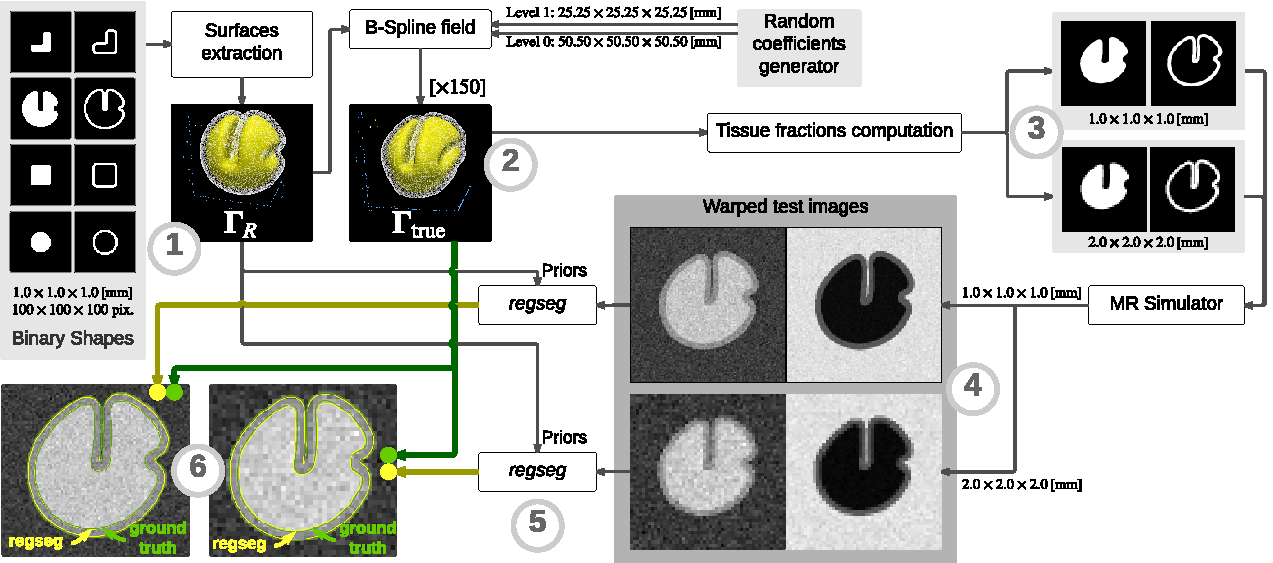
\includegraphics[width=\textwidth]{figures/figure03}
\caption{Proof of concept of the registration method. First row shows the registration experiment
  on the high-resolution ($1.0mm$ isometric) realization of the phantom, second row contains the
  low-resolution ($2.0mm$ isometric) version.
  Both phantoms were simulated with \gls*{snr} 30.
  In the first column, the distorted phantoms presented with the undistorted contours.
  For the second column, the contours have been replaced by the distorted contours using
    the ground-truth warping $U^{-1}_{true}$.
  The third column contains again the contours warped with the ground-truth field
  (thin yellow line), and the corresponding contours (green and blue thick lines)
  obtained with the presented method.
  Finally, last row represents the recovered images unwarped using the $\hat{U}_{tst}$
    found through our registration.
  }\label{fig:results_phantom}
\end{figure*}

\subsection*{Susceptibility distortion correction}
\label{sec:results_hcp}

As we propose the \gls*{fa} and the \gls*{md} as target features, we
  implemented a simplified pipeline for processing \gls*{dmri} using
  \emph{MRtrix} \citep{tournier_mrtrix_2012}.
\todo[inline]{insert here the summary of parameters}

Selecting the appropriate labels in the \emph{aparc} segmentation, we applied
  the marching-cubes algorithm again to extract priors of the following
  homogeneous regions in terms of \gls*{fa} and \gls*{md} joint distribution:
\begin{itemize}
	\item \gls*{csf} of the ventricular system,
	\item deep \gls*{gm} structures,
	\item \gls*{wm} surface as the ensemble of brain stem, and
	  cerebellar and cerebral \gls*{wm},
	\item cortical \gls*{gm} surface, including cerebellar \gls*{gm}.
\end{itemize}

\subsection*{Discussion}
\label{sec:discussion}
We propose a registration-segmentation algorithm designed for biomedical
  image analyses that are affected by all or some of the following circumstances:
  \begin{itemize}
  	\item Reference and target images do not present appropriate contrasts to
  	perform volume-based registration reliably, or there is not available an apt image
 		to be used as reference.
  	\item The low resolution of the target volume produces strong partial volume effects
  	that exclude the use of voxel-wise segmentation algorithms and hinder volume-based
  	registration.
  	\item The unknown warping is smooth enough to be represented with a sufficient number
  	of BSpline kernels, and its explicit need is justified (i.e. the distortion
  	field in \gls*{dmri} images, object tracking applications, etc.).
  \end{itemize}
The algorithm is designed for the proposed application on correcting distortions of
  \gls*{dmri} data, a required preliminary step to extract the structural connectivity
  networks.
As a consequence, our approach relies on the availability of precise segmentations or
  surfaces of the objects that are to be segmented on the target volume(s).
Connectome extraction protocols generally include the acquisition of \gls*{t1} images
  to provide with prior information about anatomy with high accuracy.
\todo[inline]{Add sentence about comment RW\#1 of IPMI2013: incorporate knowledge of
the EPI distortions into regularization}
Our method solves in a single step a joint problem usually addressed in two steps.
The first solves the linear registration of the \gls*{t1} and \gls*{dmri} data (i.e.
  \cite{greve_accurate_2009}), whereas the second corrects for the nonlinear distortions
  derived from the inhomogenety of magnetic susceptibility across tissues
  \citep{jezzard_correction_1995}.

{\color{red} We also considered the reproducibility of results a design requirement.
Therefore, real data are fetched from a publicly available repository
  (the Human Connectome Project \citep{essen_human_2012}) and all the software
  involved in this paper is also publicly released.
\autoref{fig:evworkflows} describes the general structure of the workflow we implemented
  as evaluation instrument, using \emph{nipype} \citep{gorgolewski_nipype_2011} to ensure
  reproducibility.}

We implemented the registration method upon the widely used Insight Registration and Segmentation
	Toolkit (\url{http://www.itk.org}) with the aim to release a useful and free software bundle.
The instrumentation framework is also distributed with the registration method,
  and has been implemented using \emph{nipype} \citep{gorgolewski_nipype_2011}.
The pipelines include the automatic generation of the ``cortex'' phantom.
The real datasets are publicly available under the \gls*{hcp} project.
Thus, all the experiments and results presented in this paper are intended to be
  fully reproducible.


% An example of a floating figure using the graphicx package.
% Note that \label must occur AFTER (or within) \caption.
% For figures, \caption should occur after the \includegraphics.
% Note that IEEEtran v1.7 and later has special internal code that
% is designed to preserve the operation of \label within \caption
% even when the captionsoff option is in effect. However, because
% of issues like this, it may be the safest practice to put all your
% \label just after \caption rather than within \caption{}.
%
% Reminder: the "draftcls" or "draftclsnofoot", not "draft", class
% option should be used if it is desired that the figures are to be
% displayed while in draft mode.
%
%\begin{figure}[!t]
%\centering
%\includegraphics[width=2.5in]{myfigure}
% where an .eps filename suffix will be assumed under latex, 
% and a .pdf suffix will be assumed for pdflatex; or what has been declared
% via \DeclareGraphicsExtensions.
%\caption{Simulation Results.}
%\label{fig_sim}
%\end{figure}

% Note that IEEE typically puts floats only at the top, even when this
% results in a large percentage of a column being occupied by floats.


% An example of a double column floating figure using two subfigures.
% (The subfig.sty package must be loaded for this to work.)
% The subfigure \label commands are set within each subfloat command,
% and the \label for the overall figure must come after \caption.
% \hfil is used as a separator to get equal spacing.
% Watch out that the combined width of all the subfigures on a 
% line do not exceed the text width or a line break will occur.
%
%\begin{figure*}[!t]
%\centering
%\subfloat[Case I]{\includegraphics[width=2.5in]{box}%
%\label{fig_first_case}}
%\hfil
%\subfloat[Case II]{\includegraphics[width=2.5in]{box}%
%\label{fig_second_case}}
%\caption{Simulation results.}
%\label{fig_sim}
%\end{figure*}
%
% Note that often IEEE papers with subfigures do not employ subfigure
% captions (using the optional argument to \subfloat[]), but instead will
% reference/describe all of them (a), (b), etc., within the main caption.


% An example of a floating table. Note that, for IEEE style tables, the 
% \caption command should come BEFORE the table. Table text will default to
% \footnotesize as IEEE normally uses this smaller font for tables.
% The \label must come after \caption as always.
%
%\begin{table}[!t]
%% increase table row spacing, adjust to taste
%\renewcommand{\arraystretch}{1.3}
% if using array.sty, it might be a good idea to tweak the value of
% \extrarowheight as needed to properly center the text within the cells
%\caption{An Example of a Table}
%\label{table_example}
%\centering
%% Some packages, such as MDW tools, offer better commands for making tables
%% than the plain LaTeX2e tabular which is used here.
%\begin{tabular}{|c||c|}
%\hline
%One & Two\\
%\hline
%Three & Four\\
%\hline
%\end{tabular}
%\end{table}


% Note that IEEE does not put floats in the very first column - or typically
% anywhere on the first page for that matter. Also, in-text middle ("here")
% positioning is not used. Most IEEE journals use top floats exclusively.
% Note that, LaTeX2e, unlike IEEE journals, places footnotes above bottom
% floats. This can be corrected via the \fnbelowfloat command of the
% stfloats package.

% -*- root: 00-main.tex -*-
\section*{Conclusion}
\label{sec:conclusion}

\emph{Regseg} is a variational framework to simultaneously segment and
  register 3D \gls*{dmri} data of the human brain, using within-subject
  anatomical information as reference.
The registration method segments the target multivariate image in several competing regions
  defined explicitly by their limiting surfaces.
The surfaces are active, and evolve on a free-deformation field supported by B-Splines.
A descent optimization strategy is guided by shape gradients computed on the current partition
  of the target image.
\emph{Regseg} uses active contours without edges, and hence looks for
  homogeneous regions within the image.
We tested \emph{regseg} on digital phantoms simulating \gls*{t1} and \gls*{t2} \gls*{mri},
	warped with smooth random deformations.
The resulting average misplacement of the contours was significantly lower than the
  image resolution of the phantoms.

We propose \emph{regseg} to correct \gls*{dmri} datasets for the typically present distortions
  caused by inhomogeneities of the main magnetic field.
Visual assessment of \emph{regseg} and cross-comparison with a widely-used competing
  technique demonstrated its accuracy.
Moreover, \emph{regseg} does not require additional images to the minimal acquisition protocol
  that includes only \gls*{t1} and \gls*{dmri}.

\section*{Availability and reproducibility statement}
\label{sec:availability}
We considered the reproducibility of our results a design requirement.
Therefore, we used real data fetched from a publicly available repository
  (the Human Connectome Project \citep{essen_human_2012}) and all the software
  involved in this paper is also publicly released.
The \emph{regseg} algorithm is implemented in C++, on top of ITK-4.6
  (Insight Registration and Segmentation Toolkit, \url{http://www.itk.org}).
The evaluation instruments (\autoref{fig:evworkflows}), are implemented in Python using
  \emph{nipype} \citep{gorgolewski_nipype_2011} to assess their reproducibility.
Phantom data are automatically generated by the evaluation framework.
All research elements (data, source code, figures, manuscript sources, etc.) in this paper
  are made publicly available under a unique digital object identifier in a
  package \citep{esteban_acweregistration_2015}.


% Add appendices
%% if have a single appendix:
%\appendix[Proof of the Zonklar Equations]
% or
%\appendix  % for no appendix heading
% do not use \section anymore after \appendix, only \section*
% is possibly needed

% use appendices with more than one appendix
% then use \section to start each appendix
% you must declare a \section before using any
% \subsection or using \label (\appendices by itself
% starts a section numbered zero.)
%

\appendix

\section{Proof of duality between the probabilistic and the presented frameworks}
Here the demonstration that we are preparing.

% you can choose not to have a title for an appendix
% if you want by leaving the argument blank
%\section{}
%Appendix two text goes here.

In the probabilistic approach to image segmentation, the smoothness constraints
can be introduced into the \gls{map} criterion as a \gls{mrf}. Accordingly to the
Hammersley-Clifford theorem (\textbf{FIXME}: citations needed), an \gls{mrf} can
be equivalently characterized by a Gibb's distribution:
\begin{equation}
P(\mathbf{K})=\underset{i}{\prod} Z(U)^{-1}\,e^{-U(\mathbf{x}_i \mid \beta,K)} = \mathit{const.}\,e^{- \sum\limits_i \left( U(\mathbf{x}_i \mid \beta,K) \right) } \sim e^{-\nu_B \left| K \right| }.
\end{equation}
This way, we include the assumption that the total length of the edge set $K$ is small
and we draw the equivalence with the \gls{mrf} modeling, for $U(\mathbf{x}_i \mid \beta,K)$
being the Potts model.

In the probabilistic approach, the underlying concept to segmenting an image is the
Bayes' rule. For a discrete image of $N$ pixels indexed by $i$, this rule reads as
follows:
\begin{equation}
P(K|I)=P(I \mid K)\, P(K)=\underset{i}{\prod} p (\mathbf{x}_i | K ) \, p_i(K).
\end{equation}
The normalizer probability $P(I)$ has been omitted for simplicity.

In order to express the likelihood as an absolute energy in our variation framework,
the \textit{log}-likelihood is computed:
\begin{equation}
E(K)= -\log( P(K|I) ) = \sum\limits_k \int_{\Omega_k} -\log p_k(I(\mathbf{x}),\mathbf{x}) \,d\mathbf{x}+\nu_B \left|K\right|,
\end{equation}
where $\mathbf{s} = I(\mathbf{x})$, $\mathbf{s} \in \mathbb{R}^C$ (a vector of $C$ scalar features).
Additionally, the discrete grid of $N$ pixels has been converted to a continuous space by assuming
$d\mathbf{x}$ as infinitesimal bin size.

To explicitly define the likelihood, we firstly define the squared \textit{Mahalanobis distance} that
is the exponential of a multivariate normal distribution:
\begin{equation}
\Delta^2_k (\mathbf{s}) = (\mathbf{s} - \boldsymbol{\mu}_k)^T \, \Sigma^{-1}_k \, (\mathbf{s} - \boldsymbol{\mu}_k).
\end{equation}

Therefore, the likelihood is defined as follows:
\begin{equation}
p_k(I(\mathbf{x}),\mathbf{x}) = p_k(\mathbf{s},\mathbf{x})= p_k(\mathbf{s}) = \frac{1}{ \sqrt{(2\pi)^{C}\,\left|\boldsymbol{\Sigma}_{k}\right|}}\,{e^{\left(-\frac{1}{2}  \Delta^2_k (\mathbf{s}) \right)}}.
\end{equation}

Introducing this definition on (14), we have:
\begin{equation}
E(K)= \sum\limits_k \int_{\Omega_k} -\log{\left[ \frac{1}{ \sqrt{(2\pi)^{C}\,\left|\boldsymbol{\Sigma}_{k}\right|}}\,e^{\left(-\frac{1}{2}  \Delta^2_k (\mathbf{s}) \right)} \right] } \,d\mathbf{x}+\nu_B \left|K\right|.
\end{equation}

\begin{equation}
E(K) = \sum\limits_k \int_{\Omega_k} \left( \frac{1}{2} \log{ \left( (2\pi)^{C}\,\left|\boldsymbol{\Sigma}_{k}\right| \right)} + \frac{1}{2}  \Delta^2_k (\mathbf{s}) \right) \,d\mathbf{x}+\nu_B \left|K\right|
\end{equation}

\begin{equation}
E(K) = \sum\limits_k \left( \frac{ V_k }{2} \log{ \left( (2\pi)^{C}\,\left|\boldsymbol{\Sigma}_{k}\right| \right)}+ \frac{1}{2} \int_{\Omega_k} \Delta^2_k (\mathbf{s}) \,d\mathbf{x}+\nu_B \left|K\right| \right)
\end{equation}

{\color{red} {Using the region descriptors derived in \autoref{sec:regseg-methods_map}, we propose
an \gls{adf}-like, \gls{acwe}-based, piece-wise constant, image segmentation
model (where the unknown is the deformation field)
\cite{chan_active_2001} with the energy functional obtained in
\eqref{eq:regseg-final_map_energy}. This inverse problem is ill-posed
\cite{bertero_illposed_1988,hadamard_sur_1902}.
In order to account for deformation field regularity and to render the
problem well-posed, we include limiting and regularization terms into
the energy functional \cite{morozov_linear_1975,tichonov_solution_1963}:
%
\begin{multline}
E(u) = \sum\limits_l \int_{\Omega'_l} \mdist{f}{l} \,d\vec{x} \\
+ \int \vec{u}^T \, A \, \vec{u} \, d\vec{x} + \int \tr\{(\nabla \vec{u}^T)^T B (\nabla \vec{u}^T)\} d\vec{x}
\label{eq:regseg-complete_energy}
\end{multline}
%
These regularity terms ensure that the segmenting contours in
\gls{dwi} space are still close to their native shape. The model
easily allows to incorporate inhomogeneous and anisotropic
regularization \cite{nagel_investigation_1986} to better regularize
the \gls{epi} distortion.}}

\todo[inline]{this last paragraphs in red color were located a bit
further, but I think we can keep some of the refs and still reproduce
the continuous version of the energy functional}

\section{Extensions}

\subsubsection{Semi-implicit Euler-forward optimization}
It is necessary to discretize $t$ in order to obtain a numerical
implementation of the equation \eqref{eq:regseg-gradient_final}:
\begin{align}
\frac{\vec{u}_k^{t+1}-\vec{u}_k^t}{\tau} =
&- \underset{l,m}{\sum} \underset{i}{\sum}
\left[ \mdist{f_i'}{l} - \mdist{f_i'}{m}\right]
\psi_k(\vec{c}_i)\, \hat{\vec{n}}_i \notag\\
&+2\, \boldsymbol{\alpha} \vec{u}_k^{t+1}
-2\, \boldsymbol{\beta} \Delta \vec{u}_k^{t+1}.
\end{align}

The associated Euler-Lagrange equation is found as:
\begin{equation}
(\tau^{-1} +2\, \boldsymbol{\alpha} - 2\, \boldsymbol{\beta} \Delta )\, \vec{u}_k^{t+1} =
\tau^{-1} \vec{u}_k^t - \frac{\partial}{\partial \vec{u}_k} E_{data}(\vec{u}_k^t),
\end{equation}
that is a linear system that we translate into Fourier domain,
to obtain the next deformation field $\vec{u}_k^{t+1}$:
\begin{multline}
\vec{u}_k^{t+1} = \\
 \mathcal{F}^{-1} \left\lbrace
\frac{\mathcal{F}\lbrace \tau^{-1}\vec{u}_{k}^{t} - \underset{l,m}{\sum} \underset{i}{\sum}
\left[ \mdist{f_i'}{l} - \mdist{f_i'}{m}\right] \rbrace}
     {\mathcal{F}\lbrace (\tau^{-1} +2\,\boldsymbol{\alpha})\mathcal{I} - 2\,\boldsymbol{\beta} \Delta ) \rbrace}
     \right\rbrace
\end{multline}

Here, we rewrite the Laplacian as a linear combination of the identity and shift operators:
\begin{equation}
\Delta = \sum\limits_d \mathcal{S}_d^- + \mathcal{S}_d^+ - 2 \mathcal{I}
\end{equation}
where $\mathcal{S}_{d}^{\pm}$ stands for the forward ($+$) and backward ($-$) shift
operator along coordinates axis $d$, of which the Fourier transform is found easily as
\begin{equation}
\mathcal{F}\{\mathcal{S}_{d}^{\pm}\} = e^{\pm \vec{i}\omega_{d}},
\end{equation}
where $\omega_{d}$ is the normalized pulsation along $d$-direction. Accordingly, the
Fourier transform of the discrete Laplacian is found as
\begin{equation}
\mathcal{F}\{\Delta\} = \sum\limits_d e^{-\vec{i}\omega_d } + e^{\vec{i}\omega_d } - 2 = \sum\limits_d \left( 2\cos(\omega_d) - 2 \right)
\end{equation}

The remaining transforms are trivial or can be computed using the \gls{fft}
as in \citep{estellers_efficient_2011}.

% ACKs
% -*- root: 00-main.tex -*-
% use section* for acknowledgement
\section*{Author contributions}
All the authors contributed in editing the paper.
OE implemented the method, designed and conducted the experiments, wrote the paper,
  simulated the phantoms and prepared the real data.
DZ devised and drafted the registration method, generated early phantom datasets, and
  collaborated with the implementation of the method.
AD, MBC and MJLC interpreted the results.
AD, MBC, MJLC, JPT and AS advised on all aspects of the work.

\section*{Acknowledgment}
The authors thank V. Estellers for early discussions at the beginning of this project,
  and L. A. Vese for her support during OE's research visits in her laboratory.

This study is supported by: the Spain's Ministry of Science and Innovation
  (projects TEC2010-21619- C04-03, TEC2011-28972-C02-02, CDTI-CENIT
  AMIT and INNPACTO PRECISION), Comunidad de Madrid (ARTEMIS) and
  European Regional Development Funds; the Center for Biomedical Imaging
  (CIBM) of the Geneva and Lausanne Universities and the EPFL, as well as the
  Leenaards and Louis Jeantet foundations.
DZ is supported by the Swiss National Science Foundation (SNF) under grant PBELP2-137727.



% Can use something like this to put references on a page
% by themselves when using endfloat and the captionsoff option.
\ifCLASSOPTIONcaptionsoff
  \newpage
\fi



% trigger a \newpage just before the given reference
% number - used to balance the columns on the last page
% adjust value as needed - may need to be readjusted if
% the document is modified later
%\IEEEtriggeratref{8}
% The "triggered" command can be changed if desired:
%\IEEEtriggercmd{\enlargethispage{-5in}}

% references section

% can use a bibliography generated by BibTeX as a .bbl file
% BibTeX documentation can be easily obtained at:
% http://www.ctan.org/tex-archive/biblio/bibtex/contrib/doc/
% The IEEEtran BibTeX style support page is at:
% http://www.michaelshell.org/tex/ieeetran/bibtex/
\bibliographystyle{IEEEtran}
% argument is your BibTeX string definitions and bibliography database(s)
\bibliography{ACWE}


% biography section
% 
% If you have an EPS/PDF photo (graphicx package needed) extra braces are
% needed around the contents of the optional argument to biography to prevent
% the LaTeX parser from getting confused when it sees the complicated
% \includegraphics command within an optional argument. (You could create
% your own custom macro containing the \includegraphics command to make things
% simpler here.)
%\begin{IEEEbiography}[{\includegraphics[width=1in,height=1.25in,clip,keepaspectratio]{mshell}}]{Michael Shell}
% or if you just want to reserve a space for a photo:

\begin{IEEEbiography}{Oscar Esteban}
Biography text here.
\end{IEEEbiography}

% if you will not have a photo at all:
%\begin{IEEEbiographynophoto}{John Doe}
%Biography text here.
%\end{IEEEbiographynophoto}

% insert where needed to balance the two columns on the last page with
% biographies
%\newpage

%\begin{IEEEbiographynophoto}{Jane Doe}
%Biography text here.
%\end{IEEEbiographynophoto}

% You can push biographies down or up by placing
% a \vfill before or after them. The appropriate
% use of \vfill depends on what kind of text is
% on the last page and whether or not the columns
% are being equalized.
%\vfill
% Can be used to pull up biographies so that the bottom of the last one
% is flush with the other column.
%\enlargethispage{-5in}

% that's all folks
\end{document}


